% BTL1 report — Introduction to Artificial Intelligence — English version.
% Build PDF: tectonic report/main-en.tex
\documentclass[12pt,a4paper]{article}
\usepackage{fontspec}
\usepackage{polyglossia}
\setmainlanguage{english}
\setmainfont{Liberation Serif}
\setsansfont{Liberation Sans}
\setmonofont{DejaVu Sans Mono}[Scale=0.88]
\usepackage{amsmath,amssymb}
\usepackage{booktabs}
\usepackage[margin=2.4cm]{geometry}
\usepackage{graphicx}
\usepackage{xcolor}
\usepackage{listings}
\usepackage{caption}
\usepackage[colorlinks=true,linkcolor=blue!55!black,urlcolor=blue!55!black]{hyperref}

\definecolor{codekw}{HTML}{285BC2}
\lstset{basicstyle=\ttfamily\small,columns=fullflexible,keepspaces=true,
  showstringspaces=false,keywordstyle=\color{codekw},frame=single,
  rulecolor=\color{gray!40},framerule=0.3pt,aboveskip=8pt,belowskip=8pt}

\captionsetup{font=small,labelfont=bf}
\setlength{\parskip}{2pt}

\newcommand{\code}[1]{\texttt{#1}}

\begin{document}

% ---------- Title page ----------
\begin{titlepage}
\centering
{\large\textbf{[UNIVERSITY]}\\[2pt]
\textbf{[FACULTY / DEPARTMENT]}\par}
\vspace{18mm}
{\Large\textbf{ASSIGNMENT 1 --- SEARCH}\\[4mm]
\large Semester 1, academic year 2026--2027\par}
\vspace{6mm}
{\large Course: Introduction to Artificial Intelligence\par}
\vspace{14mm}
{\huge\bfseries Pipes \& Light Up:\\[3mm]
Implementing Search Algorithms for Two Logic Puzzles\par}
\vspace{6mm}
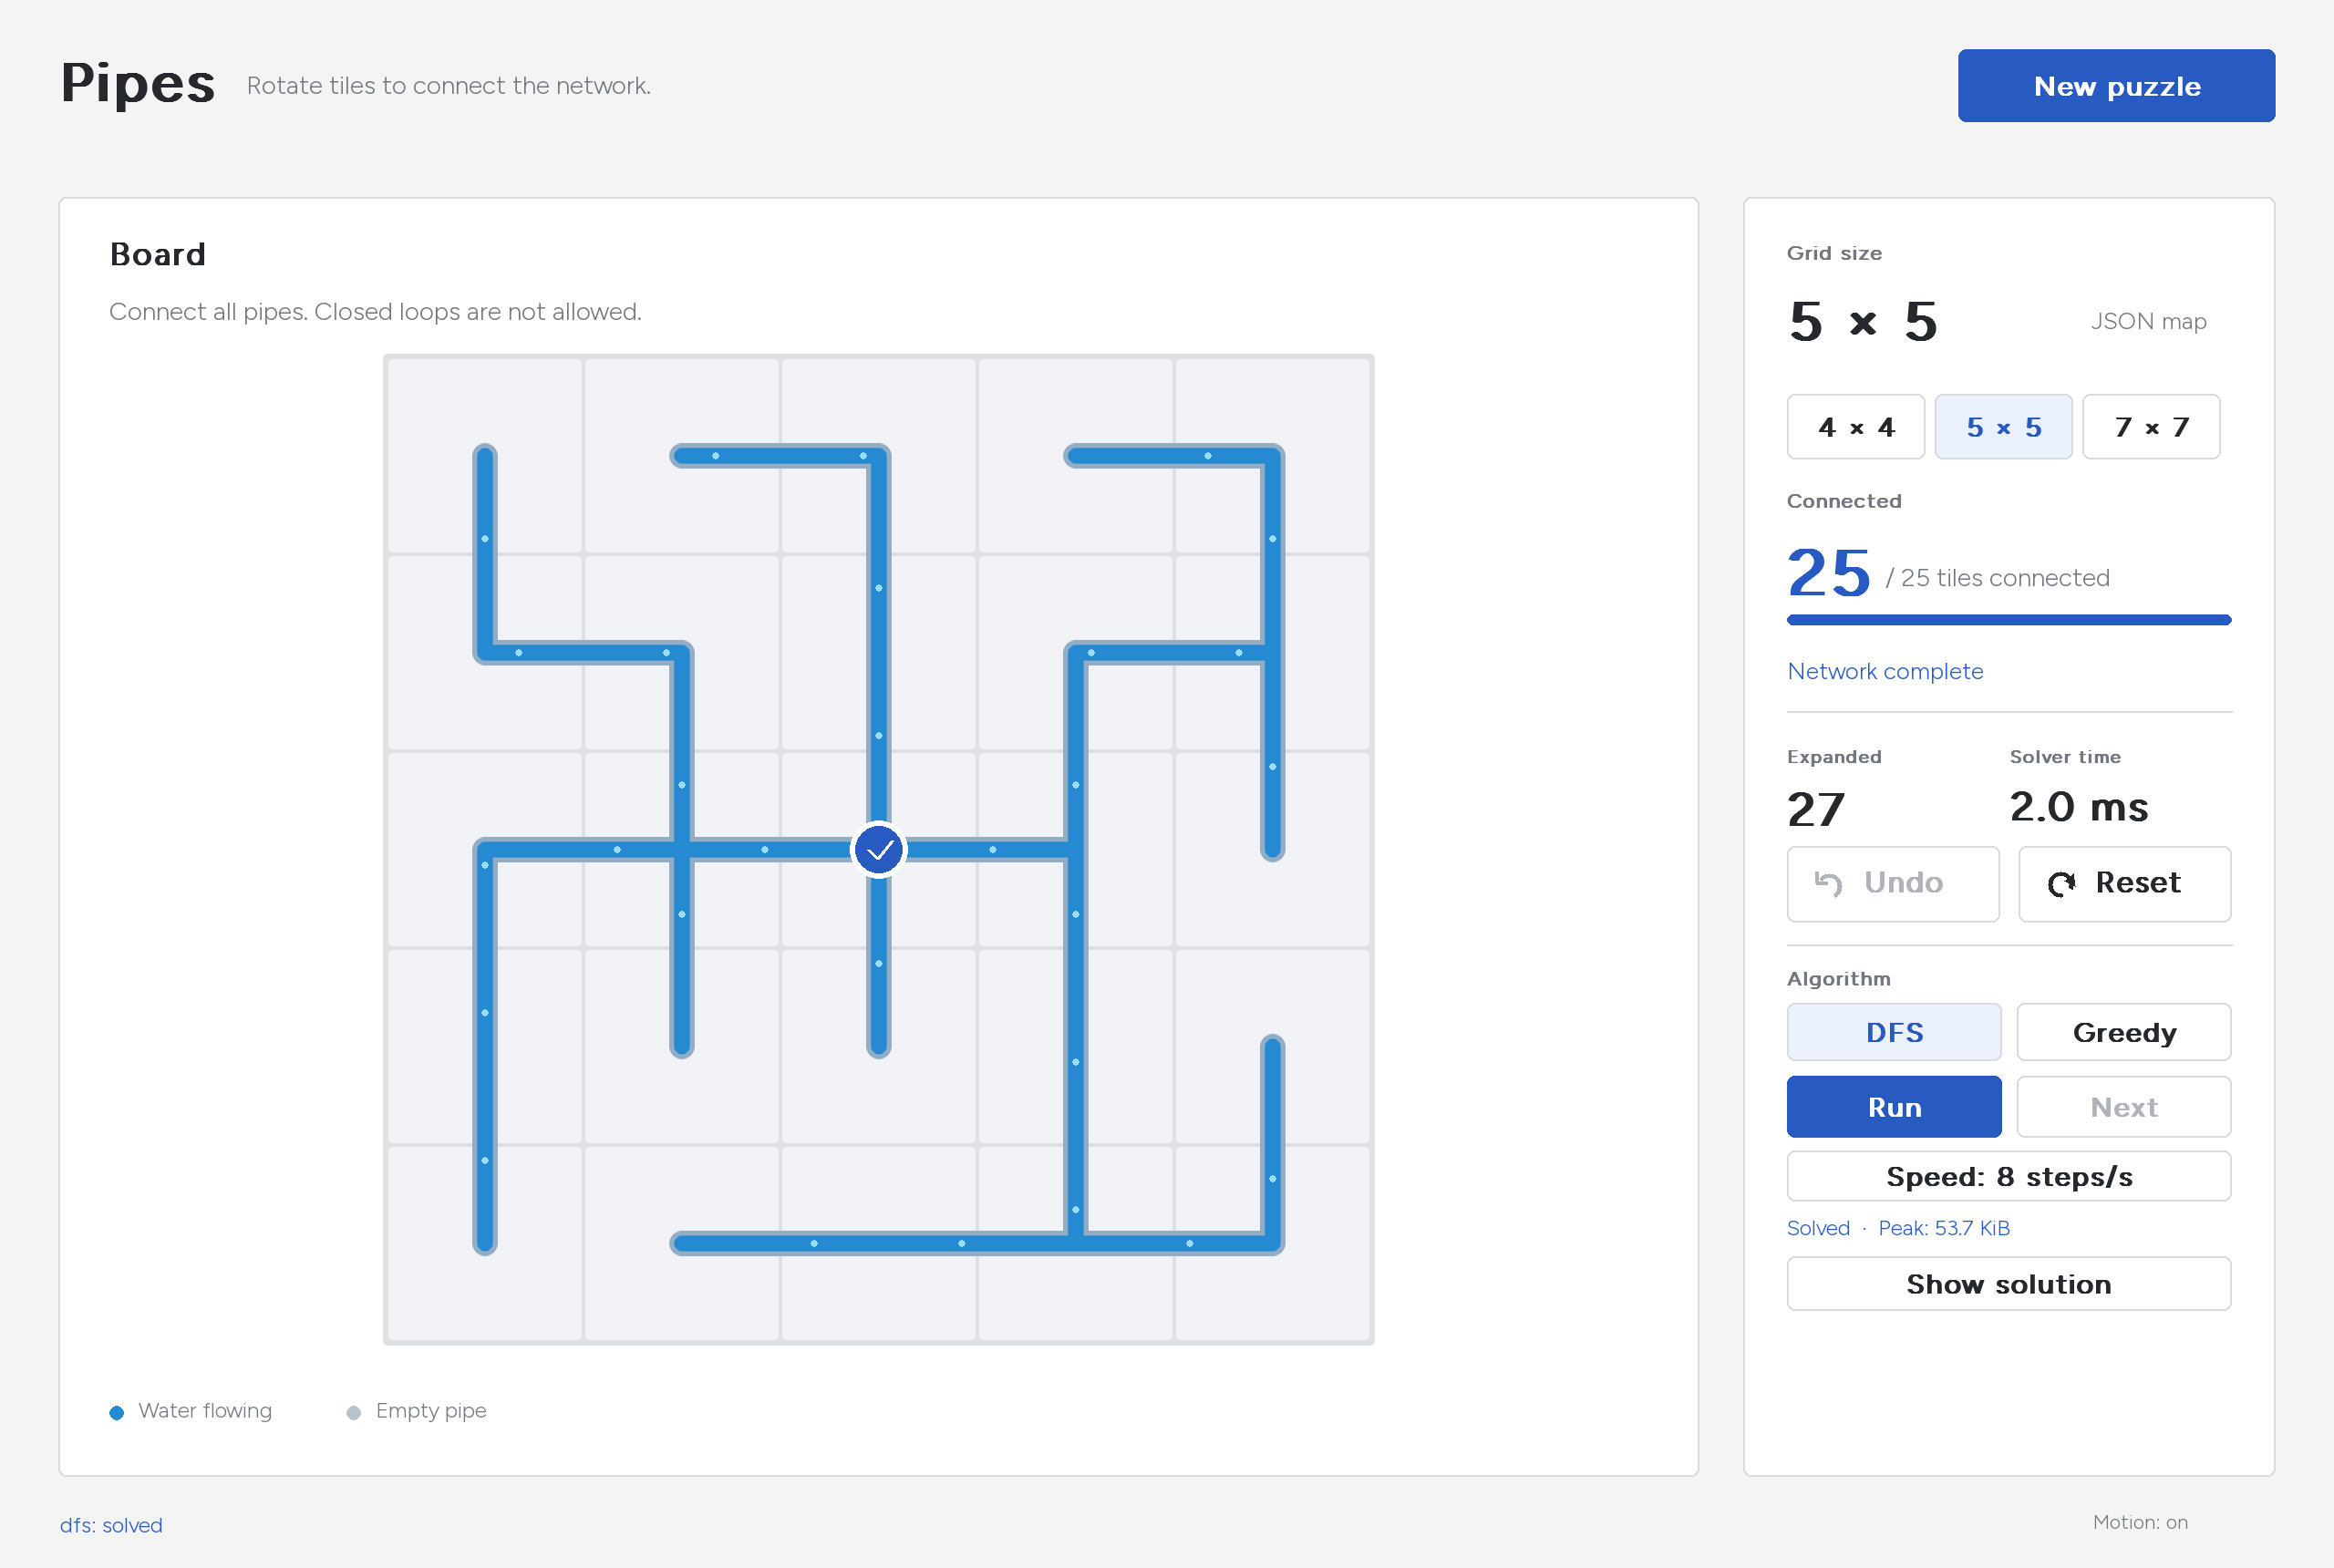
\includegraphics[width=.45\textwidth]{../docs/images/pipes.png}
\vspace{10mm}

{\large\textbf{Group members}}\par\vspace{3mm}
\begin{tabular}{@{}lll@{}}
\toprule
Full name & Student ID & Class\\
\midrule
{[Name 1]} & {[ID 1]} & {[Class 1]}\\
{[Name 2]} & {[ID 2]} & {[Class 2]}\\
{[Name 3]} & {[ID 3]} & {[Class 3]}\\
\bottomrule
\end{tabular}

\vspace{12mm}
{\large Instructor: [Instructor name]\par}
\vspace{6mm}
{\large [City], 25 October 2026\par}
\end{titlepage}

\tableofcontents
\newpage

% ---------- 1. Introduction ----------
\section{Introduction}

\subsection{Objectives}

Assignment 1 asks the group to pick two problems from the Logic Puzzles at
\url{https://www.puzzle-pipes.com/} (and related problems on that site) and
implement, in Python 3, two search algorithms for \textbf{each} problem: one
\emph{blind} search (DFS or BrFS) and one \emph{heuristic} algorithm (A*, Hill
Climbing, etc.). The submission must include a step-by-step visual demo (game
style), and a report describing how the group studied and implemented each
problem, with tables of execution time and memory consumption per algorithm per
input, and an interpretation of those numbers.

\subsection{The two chosen problems}

\begin{itemize}
\item \textbf{Pipes} (\url{https://www.puzzle-pipes.com/}): rotate pipe tiles to
form one connected, leak-free, acyclic network. Algorithms: \textbf{DFS} (blind)
and \textbf{Greedy Best-First} (heuristic).
\item \textbf{Light Up / Akari} (\url{https://www.puzzle-light-up.com/}, part of
the same Logic Puzzles family): place bulbs on white cells so that every white
cell is illuminated, no two bulbs see each other, and every numbered wall has
exactly its count of adjacent bulbs. Algorithms: \textbf{DFS} (blind) and
\textbf{A*} (heuristic, returning a minimum-bulb solution).
\end{itemize}

All four algorithms share the same state-space formulation style and were
measured on the same inputs under identical resource limits.

\subsection{Environment and tooling}

\begin{itemize}
\item \textbf{Language}: Python 3 (mandatory per the assignment). Development
uses Python 3.13 with \code{uv} for dependency management.
\item \textbf{Graphics and demo}: \code{pygame-ce} for both games;
\code{pygame-gui} adds controls to the Light Up interface.
\item \textbf{Testing and code quality}: \code{unittest} (50 tests across both
packages), \code{ruff} linting, GitHub Actions CI.
\item \textbf{Measurement}: \code{time.perf\_counter} for wall time;
\code{tracemalloc} for peak Python allocations.
\item \textbf{Documents}: \LaTeX{} (tectonic) for this report and the slides.
\end{itemize}

\subsection{Repository layout}

One shared repository, one package per puzzle:

\begin{lstlisting}
Introduction-to-AI/
  main.py             Common launcher: uv run main.py [pipes|lightup]
  pipes_problem/      Pipes game, 2 algorithms, UI, benchmark, 33 tests
  light_up_problem/   Light Up game, 2 algorithms, UI, benchmark, 17 tests
  docs/               Algorithm analysis, benchmark evidence (CSV + md)
  report/             LaTeX sources of this report (main-vi, main-en)
  slides/             LaTeX sources of the slides (main-vi, main-en)
\end{lstlisting}

Run instructions are in the repository \code{README.md}. The games start with
\code{uv run main.py pipes} and \code{uv run main.py lightup} (or
\code{python -m pipes\_problem}, \code{python -m light\_up\_problem}).

\subsection{How we studied and implemented each problem}

The group followed the same process for both puzzles:

\begin{enumerate}
\item \textbf{Learn the rules}: play the original puzzle on its official site,
note the invariants (win condition, constraints), reference
\code{puzzle-pipes.com} / \code{puzzle-light-up.com}.
\item \textbf{Formulate as search}: define state, initial state, actions,
transition model, goal test and costs; choose an efficient state representation
(orientation prefixes for Pipes, bitmasks for Light Up).
\item \textbf{Design algorithms}: one blind search (DFS) and one heuristic search
(Greedy / A*), plus a shared set of sound pruning rules; write pseudocode first.
\item \textbf{Implement and demo}: build the pygame game with a step-by-step
search visualization and solution replay.
\item \textbf{Create inputs}: write a seeded, witness-checked puzzle generator;
document the provenance of every input.
\item \textbf{Measure}: run automated benchmarks recording time, memory and node
counts to CSV; store evidence under \code{docs/benchmarks/}.
\item \textbf{Analyze}: explain the numbers, compare theory with measurement,
state limitations honestly.
\end{enumerate}

% ---------- 2. Pipes ----------
% Pipes section of the report — \input from main-vi.tex / main-en.tex.
\section{Problem 1: Pipes}

\subsection{Studying the assignment and the rules}

We studied Pipes by playing the original game at \url{https://www.puzzle-pipes.com/}
and observing its behavior. Playing first, we distilled the rules as follows:

\begin{itemize}
\item The board is an $m\times m$ grid of pipe tiles. Each tile has a \emph{fixed
shape} (straight, elbow, T-junction, cross, end) and a changeable \emph{orientation};
rotating a tile is the only move.
\item Each shape exposes ports on some of its North--East--South--West sides.
Rotation never changes the port count, only directions.
\item Goal: every open port must meet a reciprocal open port on the adjacent tile
(no port leaves the board, no dangling port), all tiles must form \textbf{one
connected} network, and the network must contain \textbf{no cycle}.
\item The water source shown in the original game is a visualization anchor: once
the network is complete, water flows from the source to every tile. Moving the
source does not change the set of valid boards.
\end{itemize}

In textbook terms this is a single-agent, deterministic, fully observable,
discrete, static task. It is a \emph{satisfaction} problem: any valid board is a
solution; minimizing manual rotations is not required (the original game does not
score rotations either).

\subsection{Search problem formulation}

Let $n=m^2$ and number the tiles in row-major order. Tile $i$ has a fixed shape
and an orientation domain $R_i$ of its distinct rotations. We formulate:

\begin{table}[h]
\centering\small
\begin{tabular}{@{}p{.20\textwidth}p{.74\textwidth}@{}}
\toprule
Component & Definition in this implementation\\
\midrule
Input & Saved scrambled board (shapes + orientations), grid size, source\\
State & Prefix $s=(a_0,\dots,a_{k-1})$ of assigned orientations\\
Initial state & Empty prefix $()$, with all tile shapes known\\
Action & Assign a boundary-valid orientation to tile $k$ (row-major order)\\
Transition & $s' = s + (a_k)$, accepted only after all feasibility checks\\
Goal test & $k=n$ and the complete board satisfies every rule\\
Cost & 1 per assignment; neither solver ranks by cost\\
Solution & One complete valid orientation tuple\\
\bottomrule
\end{tabular}
\caption{Search formulation for Pipes.}
\end{table}

One subtlety: a \emph{solver step} assigns an absolute orientation to the next
tile, while a \emph{player step} rotates a tile by 90 degrees. One assignment can
equal zero to three clicks. Both solvers share the assignment model, which makes
their comparison fair. The saved scrambled board only supplies the domains $R_i$
and the rotation order; search always starts from the empty prefix and never
reads a stored solution.

\subsection{Search space and shared pruning}

The number of complete assignments before boundary checks is
$U=\prod_i |R_i| \le 4^n$: elbows, T-junctions and ends have 4 distinct rotations,
straights 2, crosses 1. A typical 4$\times$4 board has
$U = 4^{16} \approx 4.29\times10^9$; the 7$\times$7 upper bound is
$4^{49} \approx 3.17\times10^{29}$. The assignment tree has depth $n$, branching
factor at most 4, and \textbf{every prefix has exactly one parent} (fixed
assignment order), so no closed set is needed for duplicate detection.

Orientations pointing off the board are removed up front. For each candidate
child, the shared \code{compatible()} routine applies three sound pruning layers
to both solvers:

\begin{enumerate}
\item \textbf{Match assigned neighbors}: every unassigned domain $R_i$ is
restricted to orientations matching the assigned neighbors' ports (present and
absent alike). An empty domain rejects the branch.
\item \textbf{Cycle rejection}: if assigned tiles already form a cycle, reject
(disjoint-set check).
\item \textbf{Possible connectivity}: build an \emph{optimistic} graph over tiles
--- an edge exists if some remaining orientation could open toward the other
tile. If this graph cannot connect every tile, reject.
\end{enumerate}

At the root we check the port count: a tree over $n$ vertices has exactly $n-1$
edges $=2(n-1)$ ports, and rotation preserves the count, so a different total
proves unsolvability immediately (the converse does not hold). All three layers
only remove states that cannot lead to a solution, so completeness is preserved.
DFS is therefore uninformed in its \emph{traversal order} but is a
constraint-pruned search, not a blind rotation enumerator.

\subsection{Blind search: Depth-First Search}

DFS follows the first feasible child until it reaches a goal or a dead end, then
backtracks. Rotations are enumerated in each tile's saved-orientation order ---
no heuristic information is used:

\begin{lstlisting}
SEARCH_DFS(input):
  build boundary-valid domains R_i
  if root feasibility fails: return UNSOLVABLE
  return VISIT(())

VISIT(s):
  if budget exhausted: return LIMIT_REACHED
  count one expansion
  if GOAL(s): return SOLVED(s)
  for a in boundary-valid rotations of tile |s|:
    child = s + (a)
    if FEASIBLE(child):           # 3 pruning layers
      r = VISIT(child)
      if r is SOLVED or LIMIT_REACHED: return r
  return UNSOLVABLE
\end{lstlisting}

The prefix space is finite and acyclic and the pruning is sound, so DFS is
\emph{complete} given enough resources. The first solution found does not
minimize assignments. Worst-case time is exponential in $n$; memory keeps the
current path plus pending alternatives --- this Python implementation stores
copied prefix tuples and generator frames, about $O(n^2)$ along one branch.

\subsection{Heuristic search: Greedy Best-First}

Greedy always pops from a min-heap the state with the fewest \emph{remaining
choices}:
\[
h(s) = \sum_{i \text{ unassigned}} \log_2 |D_i(s)|, \qquad
\text{priority}(s) = (h(s),\ -\text{depth}(s),\ \text{insertion order})
\]
where $D_i(s)$ is the boundary-valid domain of tile $i$ after matching assigned
neighbors. The sum is the logarithm of the product of remaining domain sizes:
domains $(1,2,4)$ give $h=0+1+2=3$, while $(1,1,2)$ give $h=1$ --- state B is
less ``free'' and is preferred. We chose this heuristic because (i) it is cheap,
reusing domains already computed during pruning, and (ii) every solution at the
same depth needs exactly $n$ assignments, so $n-k$ distinguishes nothing, while
the log-domain sum prioritizes branches that narrow fastest. $h$ is
\emph{not admissible} --- it measures remaining uncertainty, not a cost bound ---
and no $g$ term is used.

\begin{lstlisting}
SEARCH_GREEDY(input):
  build boundary-valid domains; root feasibility check
  push () into min-priority queue with priority 0
  while queue is not empty:
    if budget exhausted: return LIMIT_REACHED
    s = pop minimum-priority state;  count one expansion
    if GOAL(s): return SOLVED(s)
    for a in boundary-valid rotations of tile |s|:
      child = s + (a);  D = FEASIBLE(child)
      if D exists: push child with (h(child), -|child|, serial)
  return UNSOLVABLE
\end{lstlisting}

On the finite, acyclic prefix space, keeping all feasible candidates makes Greedy
complete given enough resources; but Greedy must hold its frontier in the heap,
so memory can grow exponentially.

\subsection{Implementation and visual demo}

The implementation lives in the \code{pipes\_problem} package: \code{model.py}
(rules, validation, board generation), \code{search.py} (both solvers, pruning,
timing and memory), \code{app.py} (pygame interface), \code{worker.py} (isolated
measurement process), \code{benchmark.py} (batch runner). The demo interface
offers:

\begin{itemize}
\item Manual play: click to rotate (Shift for counterclockwise), right-click to
lock, Undo/Reset; connected pipes carry animated blue water from the source.
\item \textbf{Step-by-step search demo}: pick DFS or Greedy, then \emph{Run /
Pause / Next / Speed}. Each event is labeled: \emph{expand} (DFS visits / Greedy
pops a prefix), \emph{assign} (DFS chooses a child), \emph{queue} (Greedy pushes),
\emph{reject} (a pruned orientation --- tile outlined in red with the reason),
\emph{backtrack}. \emph{Next} separates expansion from successor generation.
\item \emph{Show solution} replays the final assignment on its own; the board
returns to its saved state before a run. \emph{Unsolvable} and \emph{limit
reached} are distinct, explicit messages.
\end{itemize}

\subsection{Creating inputs}

Inputs are produced by the project generator (not transcribed from the web):
nine default maps covering sizes $4\times4, 5\times5, 7\times7$ with seeds
261--263, stored as compact JSON (\code{size}, \code{source}, \code{tiles}) with
the filename as the input ID. In addition, \code{maps/custom/cdai.json} is a
hand-edited \emph{unsolvable} map used to check messaging and exhausted-space
behavior. Runtime generation by \code{-{}-size}/\code{-{}-seed} is also
available. These are the team's own examples (not official website puzzle IDs),
and the generator never stores a solution in the map file.

\subsection{Experimental results: time and memory}

\textbf{Protocol.} Runs were executed on Linux x86\_64 (kernel 6.8), Python
3.13.14, pygame-ce 2.5.8. Both algorithms receive the \emph{same} nine maps, the
same row-major tile order, the same pruning, a 30-second limit and 200{,}000
expansions per run. Each (map, algorithm) pair runs 5 times: time is a headless
\code{perf\_counter} solve (no drawing); memory is the peak Python allocation
measured by \code{tracemalloc} in a separate replay, combined only when both
passes agree on status, returned board and expansion count. The full 90-run
dataset is stored at \code{docs/benchmarks/2026-10-25-pipes.csv}; the tables
below report medians per input.

\begin{table}[h]
\centering\small
\begin{tabular}{@{}llrrr@{}}
\toprule
Input & Algorithm & Solved/runs & Time (ms) & Memory (KiB)\\
\midrule
pipes-4x4-261 & DFS    & 5/5 & 3.380  & 26.836\\
              & Greedy & 5/5 & 2.866  & 11.695\\
\midrule
pipes-4x4-262 & DFS    & 5/5 & 3.047  & 27.078\\
              & Greedy & 5/5 & 3.386  & 12.359\\
\midrule
pipes-4x4-263 & DFS    & 5/5 & 3.149  & 26.984\\
              & Greedy & 5/5 & 2.741  & 12.500\\
\midrule
pipes-5x5-261 & DFS    & 5/5 & 5.352  & 53.203\\
              & Greedy & 5/5 & 7.094  & 19.500\\
\midrule
pipes-5x5-262 & DFS    & 5/5 & 5.906  & 53.344\\
              & Greedy & 5/5 & 5.882  & 19.219\\
\midrule
pipes-5x5-263 & DFS    & 5/5 & 4.564  & 53.297\\
              & Greedy & 5/5 & 5.712  & 19.219\\
\midrule
pipes-7x7-261 & DFS    & 5/5 & 23.247 & 145.852\\
              & Greedy & 5/5 & 27.049 & 27.594\\
\midrule
pipes-7x7-262 & DFS    & 5/5 & 21.938 & 145.930\\
              & Greedy & 5/5 & 26.669 & 27.070\\
\midrule
pipes-7x7-263 & DFS    & 5/5 & 40.785 & 145.852\\
              & Greedy & 5/5 & 38.246 & 29.094\\
\bottomrule
\end{tabular}
\caption{Pipes --- time and peak memory per input (median of 5 runs, measured
25 October 2026). All 90/90 runs are \emph{solved}. Source:
\code{docs/benchmarks/2026-10-25-pipes.csv}.}
\label{tab:pipes-per-input-en}
\end{table}

\begin{table}[h]
\centering\small
\begin{tabular}{@{}llrrr@{}}
\toprule
Size & Algorithm & Solved/runs & Median time (ms) & Median memory (KiB)\\
\midrule
$4\times4$ & DFS    & 15/15 & 3.149  & 26.984\\
           & Greedy & 15/15 & 3.097  & 12.359\\
$5\times5$ & DFS    & 15/15 & 5.261  & 53.297\\
           & Greedy & 15/15 & 6.157  & 19.219\\
$7\times7$ & DFS    & 15/15 & 24.469 & 145.852\\
           & Greedy & 15/15 & 31.695 & 27.594\\
\bottomrule
\end{tabular}
\caption{Pipes --- summary by board size (3 maps $\times$ 5 runs per figure).}
\label{tab:pipes-summary-en}
\end{table}

\textbf{Interpreting the results.}

\begin{itemize}
\item \textbf{Time grows quickly with size} (3--5 ms at 4$\times$4 to 22--41 ms
at 7$\times$7): variables grow from 16 to 49 and each successor's feasibility
check touches more assigned neighbors, matching the exponential prediction for
the search space.
\item \textbf{DFS is faster than Greedy at 5$\times$5 and 2 of 3 maps at
7$\times$7.} On easy inputs the pruning already steers DFS's first branch almost
straight to a solution; the priority queue only adds heap push/pop and $h$
computation without changing traversal much. This shows that a heuristic is
\emph{not free}: its bookkeeping cost must be repaid by ranking quality.
\item \textbf{On the hardest map (pipes-7x7-263) Greedy wins} (38.2 vs 40.8 ms):
this map forces real backtracking, and ranking by ``fewest remaining choices''
explores tight branches first, saving some wasted probing. The margin is small
(5\%) but appears exactly where heuristics should help.
\item \textbf{Memory: Greedy uses 4--5$\times$ less than DFS} (12--29 KiB vs
27--146 KiB). Counter to the textbook worry about Greedy's exponential frontier,
the tracemalloc figure reflects this implementation's actual Python allocations:
DFS copies a prefix tuple and holds a generator frame per recursion level, while
Greedy's frontier stays tiny on easy inputs because pruning discards almost
everything. On much harder inputs Greedy's frontier could still balloon ---
further experiments would be needed to confirm.
\item \textbf{All 90 runs solved} within limits; no run hit the 30-second or
200k-expansion budget on this input set.
\end{itemize}

\subsection{Limitations}

The default input set is quite easy under the current pruning, so neither solver
is pushed to its limits; any ``winner'' claim holds only for this kind of input.
We have not yet ablated the pruning layers separately, added many unsolvable
maps, or tried an MRV heuristic. These limitations are recorded in
\code{docs/pipes-analysis.md} as future work.


% ---------- 3. Light Up ----------
% Light Up section of the report — \input from main-vi.tex / main-en.tex.
\section{Problem 2: Light Up (Akari)}

\subsection{Studying the assignment and the rules}

We studied Light Up (also known as Akari) at
\url{https://www.puzzle-light-up.com/}, part of the same Logic Puzzles family as
Pipes. The rules, distilled by playing:

\begin{itemize}
\item The board holds \emph{white cells}, \emph{unnumbered black walls} and
\emph{numbered walls} (0--4). The task: place bulbs on white cells.
\item Each bulb shines in the four orthogonal directions until blocked by a wall
or the edge; a bulb's own cell counts as lit.
\item \textbf{Constraint 1}: every white cell must be illuminated.
\item \textbf{Constraint 2}: no two bulbs may see each other (same row/column
with no wall in between).
\item \textbf{Constraint 3}: a wall numbered $k$ must have exactly $k$
orthogonally adjacent bulbs.
\end{itemize}

Compared with Pipes, this problem adds a \emph{cost} axis: the original game's
solutions are unique (or nearly so), but the general problem admits placements
with different bulb counts. We gave the heuristic solver an optimization goal:
\textbf{A* returns a minimum-bulb solution}, while DFS returns the first solution
it finds. This difference is central to interpreting the measurements.

\subsection{Search problem formulation}

Let $W$ be the number of white cells. The single most impactful representation
decision: a state is a \textbf{$W$-bit integer bitmask} where bit $i$ means
white cell $i$ holds a bulb. Placing bulbs, checking conflicts and computing
illumination become integer operations:

\begin{table}[h]
\centering\small
\begin{tabular}{@{}p{.20\textwidth}p{.74\textwidth}@{}}
\toprule
Component & Definition in this implementation\\
\midrule
Input & Board rows: \code{None} (white), $-1$ (wall), $0..4$ (numbered wall)\\
State & Set of bulb cells, encoded as a $W$-bit bitmask\\
Initial state & Empty set (mask 0)\\
Action & Place a bulb on an eligible white cell\\
Transition & Set the cell's bit; reject successors that break rules or reachability\\
Goal test & All white cells lit, all clues exact, no bulb conflicts\\
Cost & One per placed bulb (A*'s objective)\\
Solution & A goal bulb set plus its placement order (path)\\
\bottomrule
\end{tabular}
\caption{Search formulation for Light Up.}
\end{table}

Both solvers \textbf{branch on the first unlit white cell in row-major order}:
only currently-legal bulbs that would illuminate that cell are considered. This
gives the assignment space a tree structure (one parent per state), prevents
duplicates naturally, and is \emph{identical for both solvers}, keeping the
comparison fair. Before accepting a successor, the shared \code{feasible} check
verifies: no line-of-sight conflict, no overfilled clue, every clue still able
to reach its count with legal adjacent cells, and no unlit cell left without a
possible legal illuminator. All are sound --- they only discard states that
cannot reach a goal.

\subsection{Blind search: Depth-First Search}

DFS keeps a LIFO stack of masks plus a visited set. The branching order
(``first unlit cell, row-major'') uses no heuristic information:

\begin{lstlisting}
DFS(puzzle, limits):
  push mask 0 onto the stack
  while stack is not empty:
    if budget exhausted: return TIMEOUT / NODE_LIMIT / MEMORY_LIMIT
    state = stack.pop()
    if state in visited: continue;  mark visited
    if GOAL(state): return SOLVED(state)
    cell = FIRST_UNLIT_CELL(state)        # row-major policy
    for c in legal bulbs illuminating cell:
      child = state | bit(c)
      if FEASIBLE(child): push child
  return UNSOLVABLE
\end{lstlisting}

DFS is complete on this finite space with sound pruning, but its \emph{first
solution is not minimum-cost}. Worst-case time is $O(2^W)$ states; memory holds
the visited set and the stack, also exponential in the worst case. Time, node
and memory limits end with statuses \emph{distinct} from UNSOLVABLE --- a TIMEOUT
run is not evidence of unsolvability.

\subsection{Heuristic search: A* with an admissible lower bound}

A* explores by $f(n) = g(n) + h(n)$ with $g(n)$ = bulbs placed (unit cost), a
min-heap frontier and a \code{best\_g} table that discards rediscoveries at no
better cost. The heuristic is the maximum of three lower bounds on the bulbs
still needed:

\[
h(n) = \max\left\{
\left\lceil \tfrac{D}{G_{\max}} \right\rceil,\;
\max_w d_w,\;
\left\lceil \tfrac{\sum_w d_w}{H_{\max}} \right\rceil
\right\}
\]

where $D$ = remaining dark cells, $G_{\max}$ = the most dark cells any single
legal bulb could light right now, $d_w$ = numbered wall $w$'s deficit (bulbs
still owed), and $H_{\max}$ = the most wall adjacencies one legal bulb could
satisfy simultaneously. Each component lower-bounds the remaining bulbs: one
bulb lights at most $G_{\max}$ cells; wall $w$ still needs at least $d_w$ bulbs;
the total deficit $\sum d_w$ needs at least
$\lceil \sum d_w / H_{\max}\rceil$ bulbs. The maximum of lower bounds is a lower
bound, so $h$ is \textbf{admissible}; with unit costs and a completed search,
A* returns a \textbf{minimum-bulb} solution.

\begin{lstlisting}
ASTAR(puzzle, limits):
  push (f = h(0), g = 0, mask 0) into a min-heap
  best_g = {0: 0}
  while heap is not empty:
    if budget exhausted: return TIMEOUT / NODE_LIMIT / MEMORY_LIMIT
    pop state with minimum f
    if GOAL(state): return SOLVED(state)
    for c in legal bulbs illuminating FIRST_UNLIT_CELL(state):
      child = state | bit(c)
      if FEASIBLE(child) and g+1 < best_g.get(child, inf):
        best_g[child] = g + 1
        push (g + 1 + h(child), g + 1, child)
  return UNSOLVABLE
\end{lstlisting}

The price: the heap holds the \emph{entire frontier}, the \code{best\_g} table
holds every discovered state, and each expansion recomputes three bounds over
large bitmasks. This is exactly where the measured time and memory gaps come
from.

\subsection{Implementation and visual demo}

The implementation lives in \code{light\_up\_problem}, preserving the upstream
layout: \code{core/} (board model, rules, JSON), \code{algorithms/search.py}
(both bitmask solvers), \code{generator/} (seeded boards), \code{benchmark/}
(measurement CLI), \code{ui/app.py} (pygame + pygame\_gui game), and
\code{worker.py} (spawn-safe solver process). The demo interface offers:

\begin{itemize}
\item \textbf{Manual play}: click to place or remove a bulb; lit cells are
highlighted, conflicts outlined in red, numbered walls show their current count.
\item \textbf{Step-by-step search demo}: pick DFS or A*, then Run / Pause / Step
/ Stop. Sampled \code{SearchEvent}s stream to the UI showing the current bulb
set, the focused cell, and expanded/generated/frontier counters. \emph{Play
solution} replays the returned placements one by one.
\item \textbf{Compare DFS and A*}: runs both solvers on the current puzzle and
shows time, node counts and bulb counts side by side.
\end{itemize}

\subsection{Creating inputs}

Boards are generated deterministically from a seed by
\code{generator/generate.py}: build a cyclic \emph{witness} (one bulb per row
and column), propose walls only away from witness bulbs, derive clue values from
adjacent witness bulbs, and keep a wall only if the witness remains valid. The
witness is verified with the same \code{is\_goal\_state} used during play but is
\emph{not} stored in the player-facing board. Twelve samples cover all 4 sizes
(7, 10, 14, 25) $\times$ 3 difficulties (easy/normal/hard, target wall densities
16\%/10.5\%/5.5\% of board area). Puzzles serialize as JSON in the
\code{lightup-puzzle-v1} format via \code{save\_puzzle}/\code{load\_puzzle} or
\code{-{}-puzzle-json}. Two limits are stated openly: difficulty labels are
structural (wall density), not calibrated against solve times; and solution
uniqueness is not checked.

\subsection{Experimental results: time and memory}

\textbf{Protocol.} Linux x86\_64 (kernel 6.8), Python 3.13.14 --- the same
machine as the Pipes tables. Twelve sample inputs (4 sizes $\times$ 3
difficulties), 3 repeats per algorithm, 30-second timeout, 500{,}000-node limit,
512 MB estimated-memory limit. Time is the solver's own \code{perf\_counter}
measurement; memory is the \code{tracemalloc} peak around the solver call. All
72 runs are stored at \code{docs/benchmarks/2026-10-25-lightup.csv}; the table
below reports medians of the 3 repeats. The 30-second budget is \emph{our
experimental design choice} (the assignment brief mandates no time limit),
shared by both algorithms; for the seven inputs where A* exceeded it, we reran
A* once with a 600-second budget (20$\times$) --- Table~\ref{tab:lightup-ext-en}
shows whether those runs finish, so TIMEOUT is not declared merely because the
budget was small.

\begin{table}[h]
\centering\small
\begin{tabular}{@{}lllrrrr@{}}
\toprule
Input & Algorithm & Result & Time (s) & Memory (KiB) & Nodes & Bulbs\\
\midrule
akari-7-easy & DFS    & SOLVED  & 0.0258  & 18.0   & 8    & 7\\
(7$\times$7, seed 70097) & A* & SOLVED & 0.2729 & 36.5 & 70 & 7\\
\midrule
akari-7-normal & DFS  & SOLVED  & 0.0161  & 20.0   & 9    & 8\\
(7$\times$7, seed 70194) & A* & SOLVED & 0.2355 & 63.2 & 153 & \textbf{7}\\
\midrule
akari-7-hard & DFS    & SOLVED  & 0.0271  & 23.9   & 7    & 6\\
(7$\times$7, seed 70291) & A* & SOLVED & 6.7745 & 977.8 & 3164 & 6\\
\midrule
akari-10-easy & DFS   & SOLVED  & 0.5491  & 78.3   & 248  & 11\\
(10$\times$10, seed 100097) & A* & SOLVED & 3.4994 & 184.6 & 618 & \textbf{10}\\
\midrule
akari-10-normal & DFS & SOLVED  & 0.0567  & 47.3   & 13   & 12\\
(10$\times$10, seed 100194) & A* & SOLVED & 26.6845 & 1697.7 & 5464 & \textbf{9}\\
\midrule
akari-10-hard & DFS   & SOLVED  & 0.0776  & 51.9   & 12   & 11\\
(10$\times$10, seed 100291) & A* & TIMEOUT & 30.0 & 3621.3 & 2401 & ---\\
\midrule
akari-14-easy & DFS   & SOLVED  & 0.3751  & 93.1   & 17   & 16\\
(14$\times$14, seed 140097) & A* & TIMEOUT & 30.1 & 750.9 & 347 & ---\\
\midrule
akari-14-normal & DFS & SOLVED  & 0.4228  & 101.5  & 15   & 14\\
(14$\times$14, seed 140194) & A* & TIMEOUT & 30.1 & 459.8 & 228 & ---\\
\midrule
akari-14-hard & DFS   & SOLVED  & 0.3539  & 112.5  & 17   & 16\\
(14$\times$14, seed 140291) & A* & TIMEOUT & 30.0 & 1189.1 & 363 & ---\\
\midrule
akari-25-easy & DFS   & SOLVED  & 6.6833  & 553.1  & 33   & 31\\
(25$\times$25, seed 250097) & A* & TIMEOUT & 30.3 & 483.1 & 17 & ---\\
\midrule
akari-25-normal & DFS & SOLVED  & 9.7177  & 691.5  & 35   & 34\\
(25$\times$25, seed 250194) & A* & TIMEOUT & 30.1 & 590.0 & 15 & ---\\
\midrule
akari-25-hard & DFS   & SOLVED  & 8.0858  & 824.8  & 33   & 32\\
(25$\times$25, seed 250291) & A* & TIMEOUT & 30.4 & 833.0 & 37 & ---\\
\bottomrule
\end{tabular}
\caption{Light Up --- time, memory, expanded nodes and bulbs per input (median
of 3 runs, measured 25 October 2026, shared 30-second budget). ``Bulbs'' is
\code{solution\_cost}; ``---'' marks runs that hit the limit without concluding.
All 72 runs are stored at \code{docs/benchmarks/2026-10-25-lightup.csv}.}
\label{tab:lightup-per-input-en}
\end{table}

\begin{table}[h]
\centering\small
\begin{tabular}{@{}lrrr@{}}
\toprule
Input & Time (s) & Memory (KiB) & Expanded nodes\\
\midrule
akari-10-hard (seed 100291)   & 600.0 & 72{,}003 & 151{,}546\\
akari-14-easy (seed 140097)   & 600.0 & 16{,}405 & 19{,}638\\
akari-14-normal (seed 140194) & 600.0 & 16{,}120 & 8{,}634\\
akari-14-hard (seed 140291)   & 600.0 & 31{,}244 & 9{,}477\\
akari-25-easy (seed 250097)   & 600.0 & 1{,}868  & 523\\
akari-25-normal (seed 250194) & 601.8 & 2{,}649  & 425\\
akari-25-hard (seed 250291)   & 600.2 & 9{,}121  & 1{,}359\\
\bottomrule
\end{tabular}
\caption{Light Up --- A* alone rerun with an extended 600-second budget (one
run per input) on the seven inputs that exceeded 30 s in
Table~\ref{tab:lightup-per-input-en}. \textbf{All seven runs still TIMEOUT.}
Raw data: \code{docs/benchmarks/2026-10-25-lightup-ext.csv}.}
\label{tab:lightup-ext-en}
\end{table}

\textbf{Interpreting the results.}

\begin{itemize}
\item \textbf{DFS solves all 12/12 inputs}, expanding very few nodes (7--35 on
most boards; 248 on 10-easy). The ``first unlit cell'' policy walks each branch
through the cells in order, and the shared \code{feasible} pruning rejects
conflicting bulbs early; on clue-rich boards it almost never backtracks ---
final nodes are only ~1.3$\times$ the bulb count. Time still grows with size
(0.02\,s at 7$\times$7 to 6.7--9.7\,s at 25$\times$25) mostly due to bitmask and
feasibility work over $W\approx500$--$600$ white cells, not node count.
\item \textbf{A* completes only 5/12, but every A* solution is minimum-bulb.}
On the five inputs both solvers finished, DFS matched the optimum twice
(7-easy: 7 bulbs; 7-hard: 6) and exceeded it on the other three --- most clearly
on 10-normal: DFS used 12 bulbs where A* proved 9 suffice (33\% more).
\item \textbf{A* is 9--250$\times$ slower than DFS} where it finishes (0.27 vs
0.026\,s; 26.7 vs 0.057\,s). Three cost sources: (i) the heap keeps the whole
frontier instead of one branch; (ii) every expansion recomputes three lower
bounds over bitmasks; (iii) the \code{best\_g} table fights rediscovery. A*'s
node counts are also far higher (70--5464 vs 7--13): $f$-ordering makes A*
process states DFS would never generate.
\item \textbf{Memory: A* uses 2--40$\times$ more than DFS} where it finishes,
peaking at 3621\,KiB on 10-hard before TIMEOUT --- the frontier grows exactly as
theory predicts. Notably at 25$\times$25 A*'s memory (483--833\,KiB) stays below
DFS's (553--825\,KiB): A* expands so slowly (15--37 nodes in 30 s, nearly a
second per expansion on ~500-bit masks) that it never accumulates a large
frontier, while DFS runs deep for 6--10 seconds with an accumulated visited set.
\item \textbf{TIMEOUT is not unsolvability --- and not an artifact of a
too-small 30-second budget.} We reran A* on all seven inputs with a 600-second
budget (Table~\ref{tab:lightup-ext-en}): \emph{all seven still failed to
finish}. On 10-hard alone, A* expanded 151,546 states and retained a
$\sim$70 MiB traced peak within 600 seconds while the frontier kept growing;
on the 25$\times$25 boards the per-expansion cost ($\sim$1--2 s over $\sim$500
bitmasks) means ten minutes reach only 425--1,359 states. TIMEOUT is therefore
a genuine resource-exhaustion outcome matching A*'s theoretical exponential
behavior; no run ended UNSOLVABLE (every board has a generator witness).
\end{itemize}

A note on reading the 26.68 s A* figure on 10-normal: all three repeats gave
25.4--28.0 s with \emph{exactly} 5,464 expanded nodes (the search is
deterministic), so this is real solve time, not measurement noise. A*'s
per-node cost on 10$\times$10 boards is a stable $\approx$5 ms (10-easy: 3.5 s
for 618 nodes); 10-normal is slow simply because it must expand $\approx$8.8$
\times$ more nodes --- fewer clues than 10-easy weaken the lower bounds and
widen the frontier. It sits just under the 30-second budget, while 10-hard
(fewer clues still) crosses it.

\subsection{Limitations}

Difficulty labels come from wall density rather than measured solve times, and
solution uniqueness is unverified, so no board is claimed to have a unique
solution. Memory is the tracemalloc peak of Python allocations, not process RSS.
Stronger lower bounds (for example, matching-based coverage of dark cells) were
not attempted --- such bounds could push A* further before the timeout ceiling.


% ---------- 4. Conclusion ----------
\section{Conclusion}

Both required puzzles are fully implemented: each has one blind search (DFS) and
one heuristic search (Greedy Best-First for Pipes, A* for Light Up), all in
Python 3, all with a visual step-by-step demo, and all measured for time and
memory on shared inputs under identical limits.

Lessons from the measurements:

\begin{itemize}
\item \textbf{A heuristic is not automatically faster than blind search.} On
Pipes, Greedy Best-First is slower than DFS on most easy inputs because heap
maintenance and ranking outweigh ordering benefits; it only overtakes DFS on the
hardest 7$\times$7 map. On Light Up, A* is clearly slower than DFS at 7$\times$7
--- the price of priority-queue bookkeeping and duplicate-state management in
exchange for a guaranteed minimum-bulb solution.
\item \textbf{Memory reflects frontier structure.} DFS keeps few states (path
plus current branch) while priority-queue searches must keep the whole frontier;
yet the Pipes implementation shows DFS with \emph{higher} traced memory (copied
prefixes and generator frames), while Light Up's A* shows higher memory than its
DFS (frontier plus duplicate table). Implementation details matter.
\item \textbf{State spaces grow exponentially.} Both problems hit the 30-second
ceiling on large inputs (Pipes' hardest 7$\times$7 map takes almost twice the
average; every Light Up 25$\times$25 run times out --- and even with A* rerun
at a 600-second budget, all seven over-limit Light Up inputs still fail to
finish), matching the theoretical $O(4^n)$ and $O(2^W)$ bounds.
\item \textbf{Sound pruning does the heavy lifting.} In both puzzles most of the
speed comes from correct pruning (feasibility checks, early cycle rejection,
possible-connectivity, unlightable-cell detection) rather than from traversal
order; a well-pruned blind search is already fast on small and medium inputs.
\end{itemize}

Future work: harder and provably-unsolvable inputs for broader evaluation;
per-pruning-layer ablation; uniqueness checking for Light Up; alternative
heuristics (MRV for Pipes, stronger admissible bounds for A*).

% ---------- References ----------
\begin{thebibliography}{9}
\bibitem{pipes} Puzzle Pipes. \url{https://www.puzzle-pipes.com/}
\bibitem{lightup} Puzzle Light Up (Akari). \url{https://www.puzzle-light-up.com/}
\bibitem{aima} S.~J. Russell, P.~Norvig, \emph{Artificial Intelligence: A Modern
Approach}, 4th edition, Pearson, 2021 (Chapter 3: Searching; Chapter 6:
Constraint Satisfaction Problems).
\bibitem{pydoc} Python 3 documentation: \code{time}, \code{tracemalloc},
\code{multiprocessing}, \code{heapq}, \code{unittest}.
\url{https://docs.python.org/3/}
\bibitem{pygame} pygame-ce documentation. \url{https://pyga.me/docs/}
\quad pygame\_gui documentation. \url{https://pygame-gui.readthedocs.io/}
\end{thebibliography}

\end{document}
